\documentclass[../main]{subfiles}
\begin{document}

\chapter{半双工调频无线对讲机}%
\label{cha:半双工调频无线对讲机}

\section{实验目的}%
\label{sec:\arabic{chapter}实验目的}

\begin{enumerate}

	\item 在模块实验的基础上掌握调频发射机、接收机,整机组成原理,建立调频系
		统概念;

	\item 掌握系统联调的方法,培养解决实际问题的能力。

\end{enumerate}

\section{实验任务}%
\label{sec:\arabic{chapter}实验任务}

\begin{enumerate}

	\item 完成调频发射机整机联调;

	\item 完成调频接收机整机联调;

	\item 进行调频发送与接收系统联调。

\end{enumerate}

\section{基本原理}%
\label{sec:\arabic{chapter}基本原理}

\begin{figure}[htbp]
	\centering
	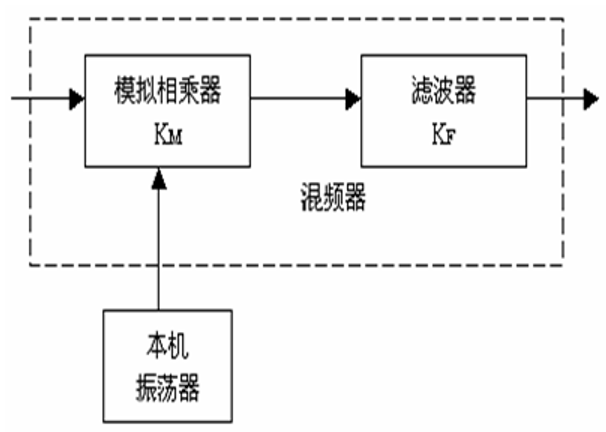
\includegraphics[width=0.8\linewidth]{block.png}
	\caption{半双工调频无线对讲机系统框图}
	\label{fig:半双工调频无线对讲机系统框图}
\end{figure}

该调频发射、接收机组成原理框图如图\ref{fig:半双工调频无线对讲机系统框图} 所示,
发射机由音频信号发生器,音频放大,调频、上变频、功放等电路组成。接收机则由高放,
下变频、中频放大、限幅、FM解调、音频功放、耳机等部分组成。

\section{实验步骤}%
\label{sec:\arabic{chapter}实验步骤}

\subsection{FM发射机实验}%
\label{sub:FM发射机实验}

在做本实验前请调试好与本实验相关的各单元模块.

\begin{enumerate}

	\item 将模块1的$ S_6 $拨上,即选通音乐信号,经$ U_4 $放大从$ J_5 $口输出
		,调节 $ W_3 $ 使$ J_5 $口处信号为最大不失真状态。

	\item 将模块1的$ J_5 $口通过开关$ S_5 $切换连接到模块1的J2口,$
		\mathrm{TH}_2 $处测试音乐信号,将模块1的$ S_1 $、$ S_3 $均拨上,
		调节$ \mathrm{CC}_1 $使$ J_1 $端输出频率接近$ 4.5MHz $的调频信号
		(可在$ \mathrm{TH}_1 $处观测),调节$ W_2 $和中周$ T_1 $使波形
		达到最大不失真状态。

	\item 将模块1的$ J_1 $连接到模块2的$ J_6 $,另将信号源频率\SI{8}{\MHz}
		( $ V_\mathrm{P-P}\approx\SI{500}{\mV} $)的信号从模块2的$ J_7
		$口输入,经平衡混频可得到\SI{12.5}{\MHz}左右的高频信号(可在$
		\mathrm{TH}_9 $ 处观测)。

	\item 将模块2的$ J_8 $口连到模块3的$ J_3 $口,从$ \mathrm{TH}_5 $可观测
		到放大后的\SI{12.5}{\MHz}高频信号,将已放大的高频信号从模块3的$
		S_4 $ 切换拨上送到天线发送出去。

\end{enumerate}

\begin{figure}[htbp]
	\centering
	\begin{subfigure}[htbp]{.45\linewidth}
		\centering
		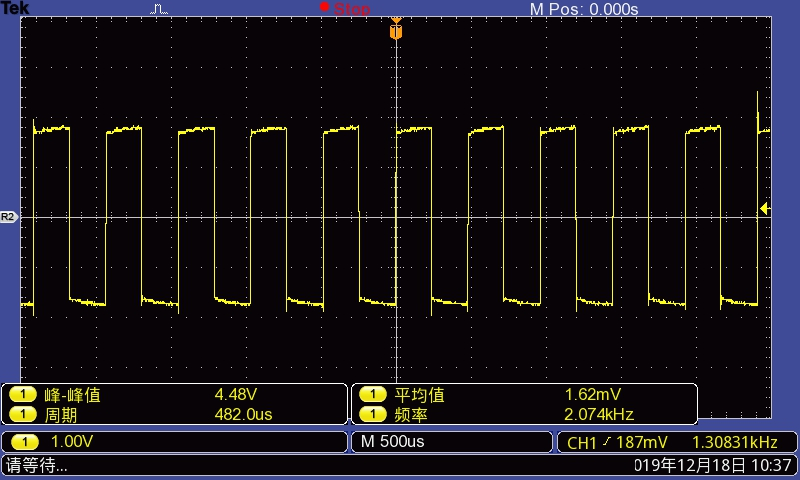
\includegraphics[width = \linewidth]{TP11.JPG}
		\caption{TP11音源输入}
		\label{fig:TP11音源输入}
	\end{subfigure}
	\quad
	\begin{subfigure}[htbp]{.45\linewidth}
		\centering
		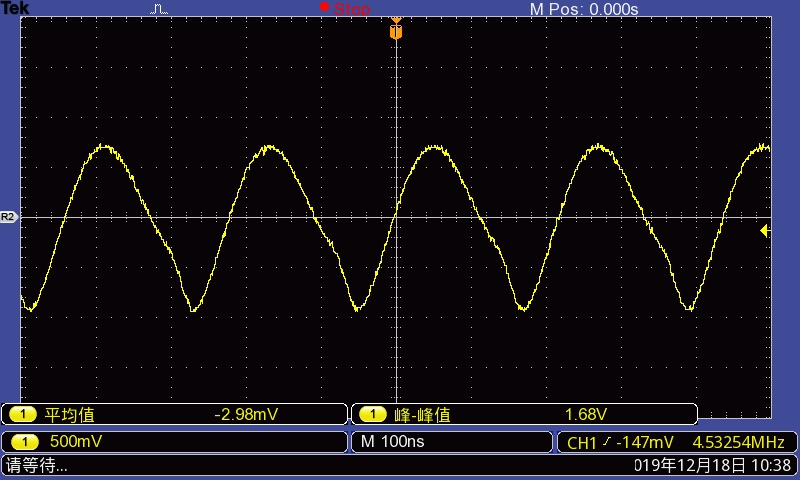
\includegraphics[width = \linewidth]{TP1.JPG}
		\caption{TP1调频输入}
		\label{fig:TP1调频输入}
	\end{subfigure}

	\begin{subfigure}[htbp]{.45\linewidth}
		\centering
		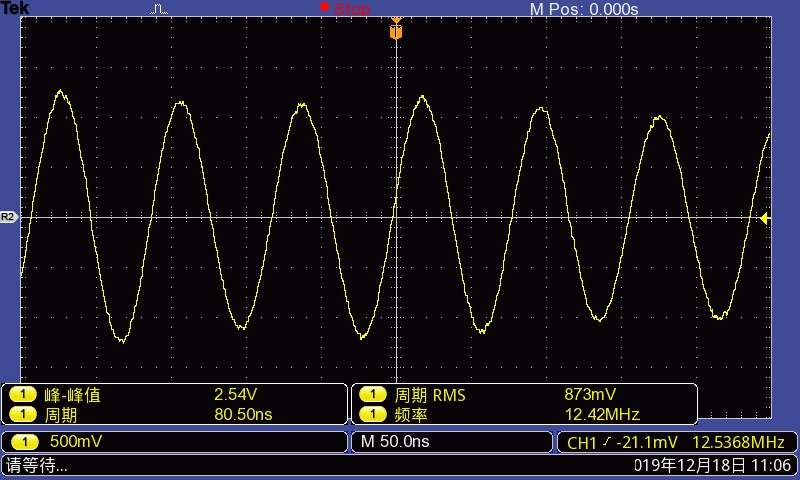
\includegraphics[width = \linewidth]{up-12-5.JPG}
		\caption{上变频12.5MHz}
		\label{fig:上变频12.5MHz}
	\end{subfigure}
	\quad
	\begin{subfigure}[htbp]{.45\linewidth}
		\centering
		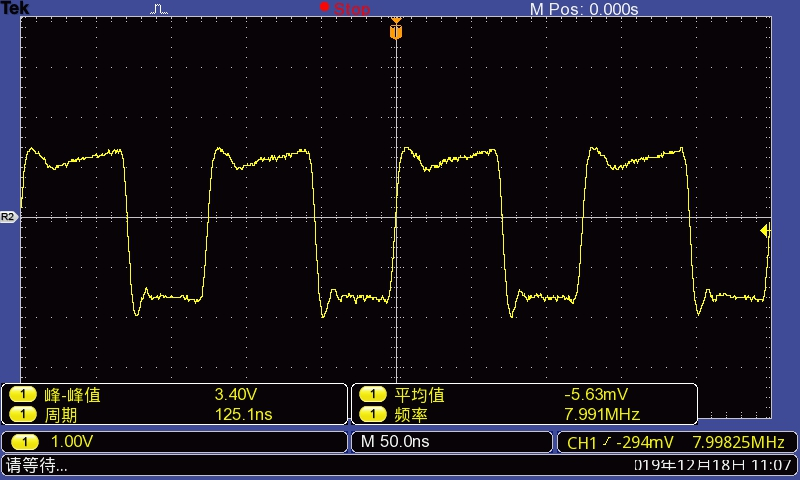
\includegraphics[width = \linewidth]{up-8.JPG}
		\caption{上变频8MHz}
		\label{fig:上变频8MHz}
	\end{subfigure}

	\begin{subfigure}[htbp]{.45\linewidth}
		\centering
		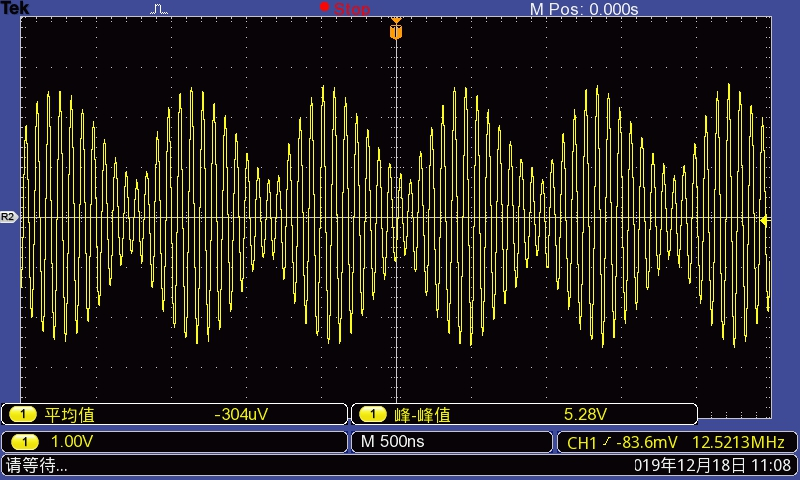
\includegraphics[width = \linewidth]{TP7.JPG}
		\caption{TP7功放}
		\label{fig:TP7功放}
	\end{subfigure}
	\caption{接收机}
	\label{fig:接收机}
\end{figure}

\subsection{FM接收机实验}%
\label{sub:FM接收机实验}

\begin{enumerate}

	\item 将模块1天线接收到的信号通过$ S_7 $开关切换送入到模块1的$ J_3 $,从
		$ \mathrm{TH}_4 $处可观测到放大后的天线接收到的信号,将放大的高
		频信号从模块1的$ J_4 $连接到模块2的$ J_3 $,将信号源频率为
		\SI{8}{\MHz}的本振信号(约\SI{500}{\mV}左右)从模块2的$ J_4 $输
		入,调整本振频率使得混频输出为\SI{4.5}{\MHz}的中频信号(可在$
		\mathrm{TH}_6 $ 处观测)。

	\item 将混频后的信号从$ J_5 $处送入模块2的$ J_1 $端口,可在$
		\mathrm{TH}_3 $处观测到经选频放大后的\SI{4.5}{\MHz}中频信号,放
		大后的中频信号从模块2的$ J_2 $口输出。

	\item 将模块2的$ J_2 $连到模块4的正交鉴频的输入端$ J_6 $,适当调节$ L_1
		$ ,可从$ \mathrm{TH}_7 $ 处观测到解调后的信号。

	\item 将模块4的$ J_7 $连到模块4的$ J_{11} $,经放大后的信号从模块4的$
		J_{12} $口连接到模块6 的$ J_6 $口输入到喇叭,可适当调节模块4的$
		W_1 $ 和模块4 的$ L_1 $,使耳机听到的声音音质清晰。

\end{enumerate}

\begin{figure}[htbp]
	\centering
	\begin{subfigure}[htbp]{.45\linewidth}
		\centering
		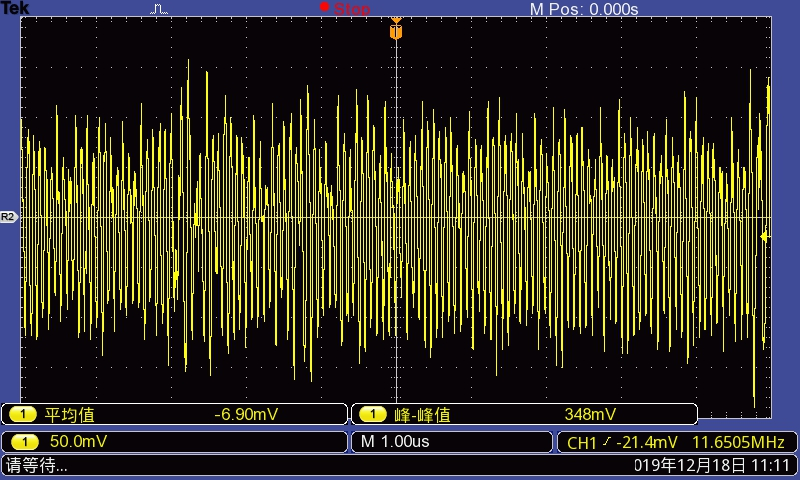
\includegraphics[width = \linewidth]{TP3.JPG}
		\caption{TP3输出}
		\label{fig:TP3输出}
	\end{subfigure}
	\quad
	\begin{subfigure}[htbp]{.45\linewidth}
		\centering
		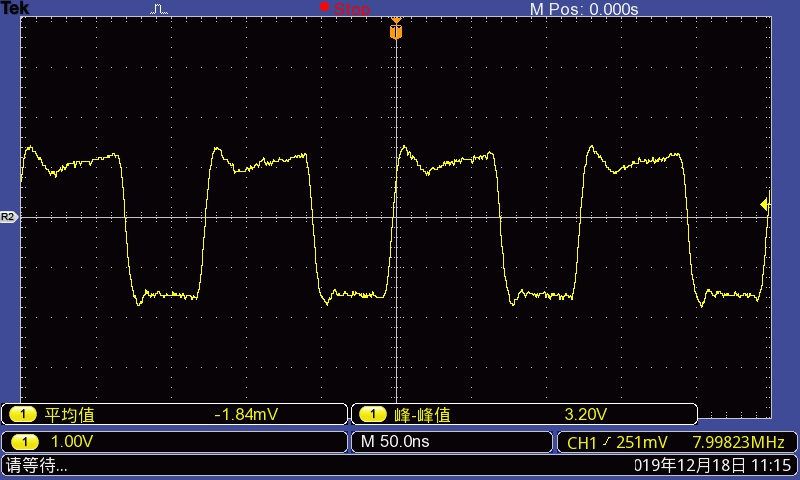
\includegraphics[width = \linewidth]{down-8.JPG}
		\caption{下变频8MHz}
		\label{fig:下变频8MHz}
	\end{subfigure}

	\begin{subfigure}[htbp]{.45\linewidth}
		\centering
		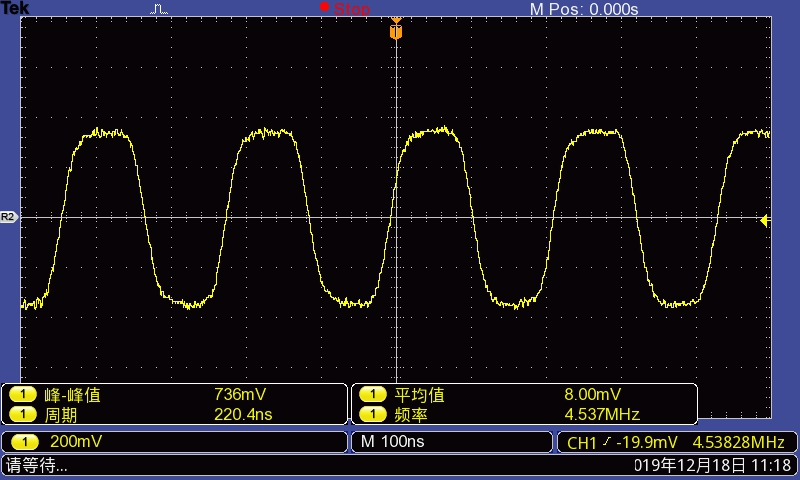
\includegraphics[width = \linewidth]{I.JPG}
		\caption{中频放大}
		\label{fig:中频放大}
	\end{subfigure}
	\quad
	\begin{subfigure}[htbp]{.45\linewidth}
		\centering
		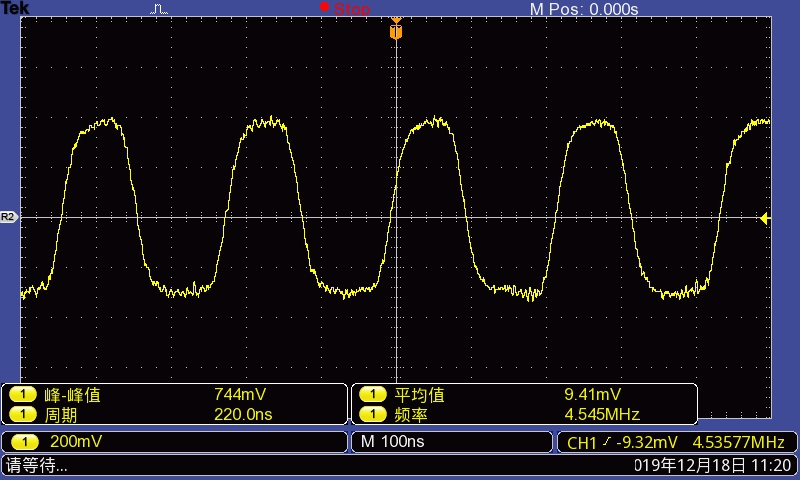
\includegraphics[width = \linewidth]{TP8.JPG}
		\caption{TP8解调}
		\label{fig:TP8解调}
	\end{subfigure}

	\begin{subfigure}[htbp]{.45\linewidth}
		\centering
		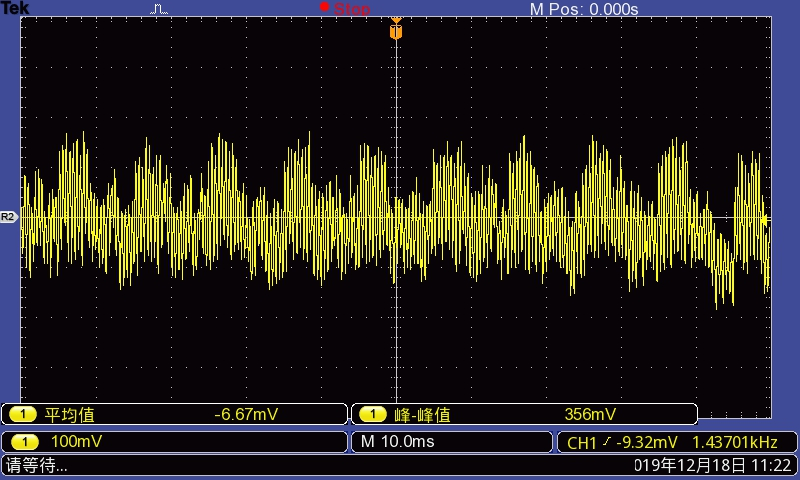
\includegraphics[width = \linewidth]{TP10.JPG}
		\caption{TP10功放}
		\label{fig:TP10功放}
	\end{subfigure}
	\quad
	\begin{subfigure}[htbp]{.45\linewidth}
		\centering
		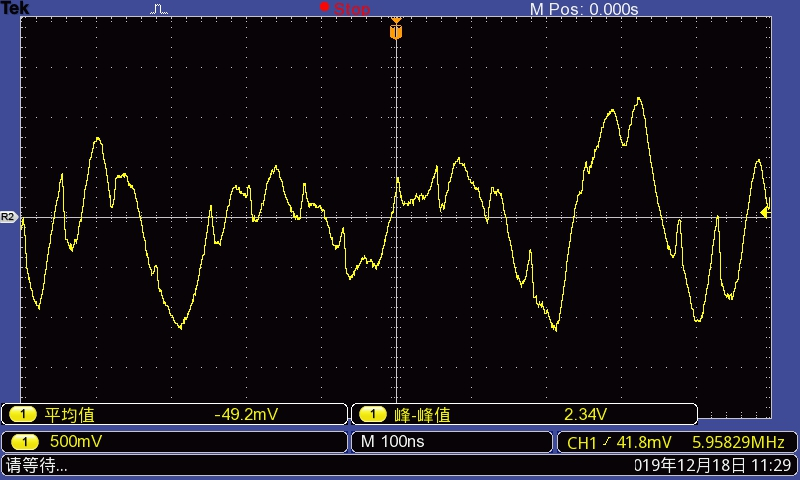
\includegraphics[width = \linewidth]{down-4-5.JPG}
		\caption{下变频4.5MHz}
		\label{fig:下变频4.5MHz}
	\end{subfigure}
	\caption{FM接收机实验}
	\label{fig:FM接收机实验}
\end{figure}

\subsection{调频系统联调}%
\label{sub:调频系统联调}

发射机实验中步骤4中模块2的$ J_8 $直接连到接收机实验中的步骤1中模块2的$ J_4 $,接
收机的本振共用发射机的本振,其它步骤不变。即可完成调频系统发射,接收实验。

\section{实验报告要求}%
\label{sec:\arabic{chapter}实验报告要求}

\begin{Exercise}

	写出实验目的和任务。

\end{Exercise}

\begin{Answer}

	实验目的见章节\ref{sec:\arabic{chapter}实验目的},实验任务见章节
	\ref{sec:\arabic{chapter}实验任务}。

\end{Answer}

\begin{Exercise}

	画出调频发射机组成框图对应点的实测波形和大小。

\end{Exercise}

\begin{Answer}

	调频发射机组成框图对应点的实测波形见图\ref{fig:接收机}。

\end{Answer}

\begin{Exercise}

	写出调试中遇到的问题,并分析说明。

\end{Exercise}

\begin{Answer}

	\begin{enumerate}

		\item 天线接触不良,信号传输不畅,无法达到效果,我们通过双手捏紧
			两根天线并保持接触解决这一问题;

		\item 混频器产生的\SI{12.5}{\MHz}信号频率不稳,振幅太小,导致无
			线发送端的信号振偏太小,检测不出来。我们重新对中周进行了
			调节,最终使频率稳定;

		\item 由于模块四中的鉴频电路中的电感$ L_1 $调节不合适,导致音乐
			声音很小,经过重新调节,问题得以解决。

	\end{enumerate}

\end{Answer}

\section{实验仪器}%
\label{sec:\arabic{chapter}实验仪器}

\begin{table}[htbp]
	\centering
	\caption{实验仪器}
	\label{tab:\arabic{chapter}实验仪器}
	\csvautobooktabular{tab/\arabic{chapter}/BOM.csv}
\end{table}

\end{document}

